
\subsubsection{Case Study: GHCN}
\textcolor{red}{Moved \& walked through b/c was getting clunky to not have terms yet}\\

Lets say we are working with the Global Historical Climatology Network\cite{AnOverviewoftheGlobalHistoricalClimatologyNetworkDailyDatabase}, which is a dataset of global daily meterological observations. Each record includes the timestamp, location, and measurements such as temperature, precipitation, and snowfall.
% can't make a 1D fiber - can't make a 1D fiber, switch the picture to plane over 0D and 1D and then can talk about disconnected or connected

% break out the mbox/clean up the typesetting
The fiber bundle model is flexible enough to express some of the many different forms that temperature data can come in. 

\begin{figure}[ht!]
    \begin{subfigure}{.5\textwidth}
        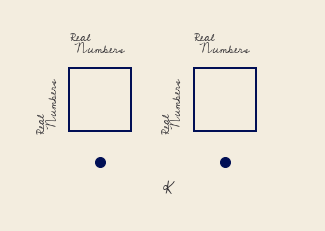
\includegraphics[width=\textwidth]{figures/math/temp_1k.png}
        %% add box around neighboring P and Map
        \label{fig:base_example_line}
    \end{subfigure}
    \begin{subfigure}{.5\textwidth}
        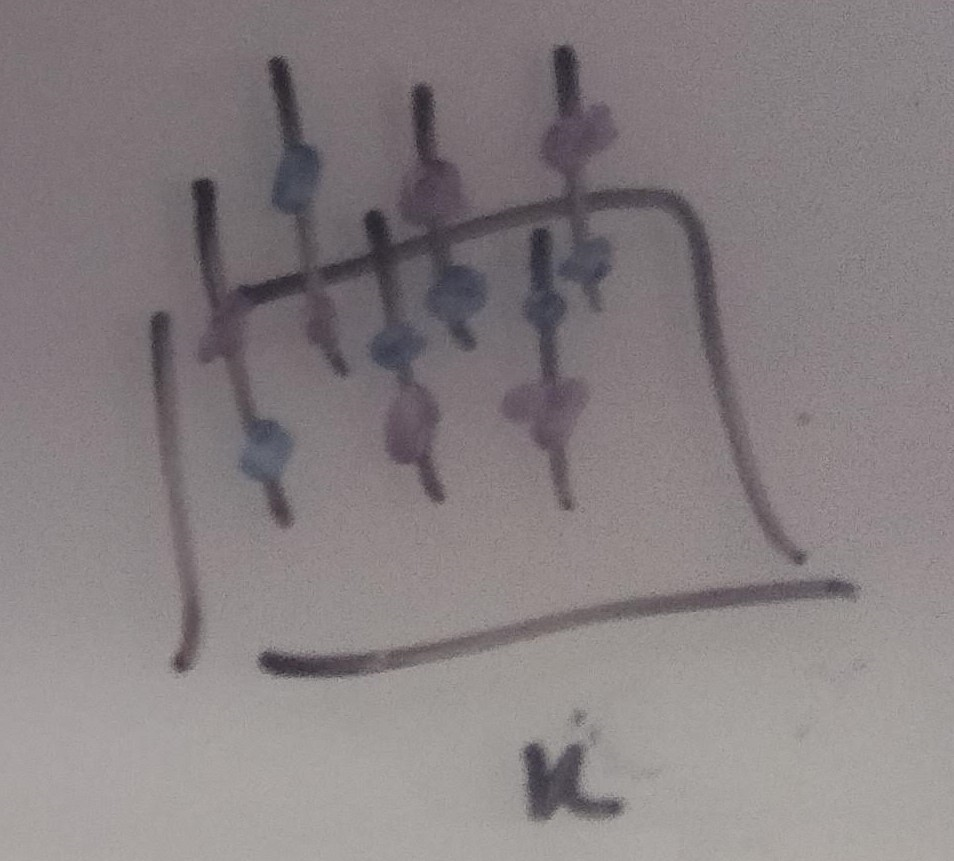
\includegraphics[width=\textwidth]{figures/math/temp_2k.png}
        \label{fig:base_example_plane}
    \end{subfigure}
    \label{fig:base_example}
    \caption{These two datasets have the same fiber of temperature but different base spaces. In figure~\ref{fig:base_example_line} the temperature values are 1D continuous, while in figure~\ref{fig:base_example_plane} the temperature values are 2D continuous.}
\end{figure}

The datasets in figure~\ref{fig:base_example} have identical fibers that encode a set of temperature values. In figure~\ref{fig:base_example_line} the temperatures lie on a line such that a section could return a timeseries or a distribution. In figure~\ref{fig:base_example_plane}, the temperatures lie on a 2D continuous plane; a section could return a map or contour. Because the fiber is 1D, it does not encode metadata 

\begin{figure}[ht!]
    \begin{subfigure}{.5\textwidth}
        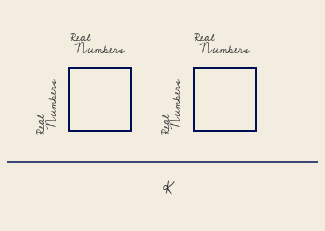
\includegraphics[width=\textwidth]{figures/math/temp_2f.png}
        \label{fig:fiber_example_plane}
    \end{subfigure}
    \begin{subfigure}{.5\textwidth}
        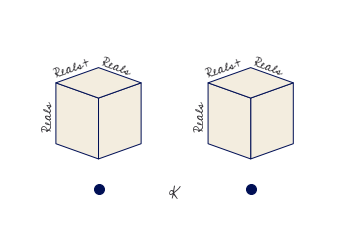
\includegraphics[width=\textwidth]{figures/math/temp_3f.png}
        \label{fig:fiber_example_cube}
    \end{subfigure}
    \label{fig:fiber_example}
    \caption{The fiber is expanded to include metadata fields that describe the semantics of $K$. In figure~\ref{fig:fiber_example_plane} the fiber is \textrm{temperature} $\times$ \textrm{time} and in figure~\ref{fig:fiber_example_cube} the fiber is \textrm{temperature}$\times$ \textrm{latitude} $\times$ {longitude}}.
\end{figure}

To encode the metadata, the fiber is expanded as illustrated in figure~\ref{fig:fiber_example}. The fiber in figure~\ref{fig:fiber_example_plane} is the cartesian product of the space of possible temperature values in degrees celsius and space of possible time values
\begin{equation}
F = [temp_{min}, temp_{max}] \times [time_{min}, time_{max}]
\label{eq:fiber_plane}
\end{equation}

while the fiber in figure~\ref{fig:fiber_example_cube} is the cartesian product of temperature, latitude, and longitude
\begin{equation}
F = [temp_{min}, temp_{max}] \times [-90, 90] \times [-180, 180]
\label{eg:fiber_cube}
\end{equation}

such that $E$ is the space of all possible points in $F$.

\begin{figure}[ht!]
    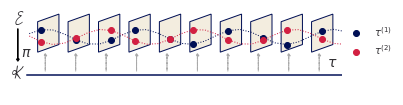
\includegraphics[width=1\linewidth]{figures/math/fiberbundle.png}
    \label{fig:fiber_example_section}
    \caption{The section $\tau_1$ returns the blue points,  while $\tau_2$ returns the purple points. $\Gamma(E)$ is the set of all sections, including $\tau_1$ and $\tau_2$}.  
\end{figure}
Given the fiber described in equation~\ref{eq:fiber_plane}, the sections $\tau_{1}$ and $\tau_{2}$ in figure~\ref{fig:fiber_example_section} return tuples of the form
\begin{equation}
\tau(k) = (k, (temperature, time))
\end{equation}
such that sections with the constraint that time is monotonic return a timeseries. 

\begin{figure}[ht!]
    
\includegraphics[width=\textwidth]{figures/math/rotation_actions.png}
    \label{fig:data_monoid_rotation}
    \caption{The set of rotation actions [turn 0, 90, 180] on the star produce a star (closed), include a rotation that does not change the orientation (identity), and can be done in any order to produce the same final orientation (closure); therefore the rotations are a set of monoid actions.
    %% dataset that is symmetric, fiber is x,y, rotatation action
    %% rotate + plot or plot + rotate
    %%emoji shuffle 
    }  
\end{figure}

\begin{figure}[ht!]
    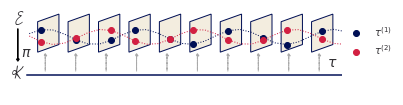
\includegraphics[width=.5\linewidth]{figures/math/fiberbundle.png}
  
    \caption{ The fiber $F$ is a continuous plane encoding the set of all possible (time, temperature) values.  The base space $K$ expresses that the fibers lie in continous space and therefore the data is continuous. The mapping $\pi:E\rightarrow K$ from total space to base space is what defines this structure as a fiber bundle. The continuous function $\tau_1$ returns a record in each fiber for each point on $K$; the set of all values $\tau_1$ returns is a dataset that lies in this fiberbundle. \note{remove one of the sections from this figure/maybe kill this example}}
    \label{fig:data_base_space} 
\end{figure}
The fiber bundle in figure~\ref{fig:data_base_space} is a representation of continuous (temperature, time) data. The fiber bundle abstraction facilitates seperately representing the time and temperature variables in the fiber $F$ and how these variables are connected in the base space $K$.  The function $\tau_1$ returns a record (temperature, time) for ever point on the interval $K$ and there can be many $\tau$ functions in the fiber bundle. 
